% Hasse diagram for PS1 Q14 (Satyajit): arrows go from coarser to finer.
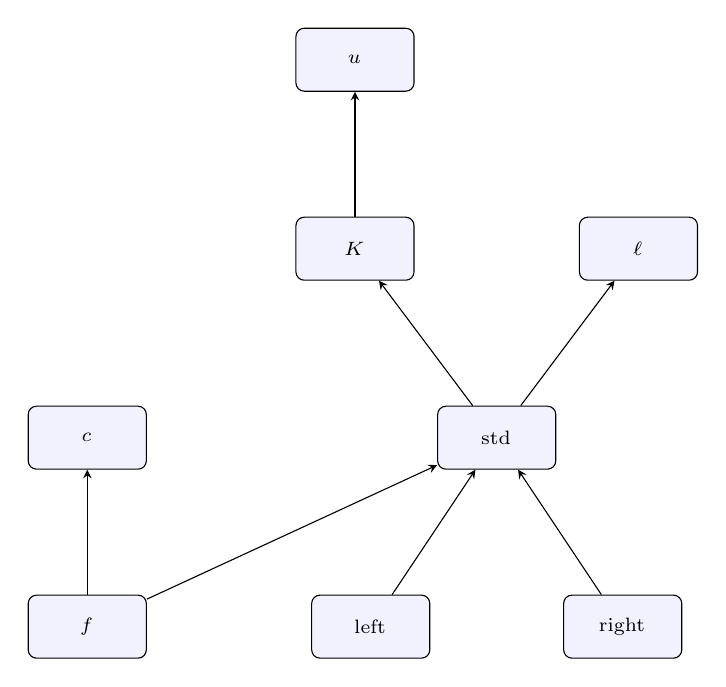
\begin{tikzpicture}[>=stealth,node distance=1cm,
  t/.style={draw,rounded corners=3pt,minimum width=1.5cm,minimum height=0.8cm,fill=blue!5}]
  \node[t] (f)  at (-5.2,0)   {$\T_f$};
  \node[t] (c)  at (-5.2,2.4) {$\T_c$};
  \node[t] (le) at (-1.6,0)   {$\T_{\mathrm{left}}$};
  \node[t] (ri) at (1.6,0)    {$\T_{\mathrm{right}}$};
  \node[t] (st) at (0,2.4)    {$\T_{\mathrm{std}}$};
  \node[t] (k)  at (-1.8,4.8) {$\T_K$};
  \node[t] (l)  at (1.8,4.8)  {$\T_\ell$};
  \node[t] (u)  at (-1.8,7.2) {$\T_u$};
  \draw[->] (f) -- (c);
  \draw[->] (f) -- (st);
  \draw[->] (le) -- (st);
  \draw[->] (ri) -- (st);
  \draw[->] (st) -- (k);
  \draw[->] (st) -- (l);
  \draw[->] (k) -- (u);
\end{tikzpicture}
